As described in Section \ref{sec:controller}, only the longitudinal motions are controlled by reinforcement learning agents. This section explains the experiments performed to test the proposed control system in the longitudinal plane, while keeping lateral motions to a minimum. Throughout all phases, the lateral motion controller had the task of keeping the deviation in lateral path distance and heading angle at a minimum. This was done by supplying the lateral PID controller with the references shown in Eq. \eqref{eq:lateral_references}.
\begin{equation} \label{eq:lateral_references}
    y_{ref} = 0 \qquad \psi_{ref} = 0 \qquad \phi_{ref} = \phi_{trim}
\end{equation}

The experiment consisted of two phases: an (online) training phase and a test phase. The training phase consisted of two parts. First, a training scenario was designed that could reliably allow the reinforcement learning controller to converge while containing sufficiently aggressive maneuvers for real scenarios. Next, the optimal training hyperparameters  for training were determined by means of a grid search over various hyperparameter combinations and random seeds. For the test phase, two maneuvers were designed to push the limits of the newly trained controller. 

\subsection{Training phase} \label{ssec:trainingphase}

In the training phase, the RL controller is asked to perform basic control tasks of increasing difficulty in order to achieve a certain baseline performance. To that end, the cyclic and collective agents were trained semi-separated from each other for 120 seconds in total. The environment is initialized at level, low-speed cruise, $V_{tas} = 15\si[per-mode=symbol]{\meter \per \second}$. For the first 60 seconds, the cyclic is training while the collective is controlled by a PID controller that is tasked with keeping a constant altitude. In the second minute, the collective is actively trained while the cyclic fine-tunes. 

The reference signal is as follows. 
The cyclic controller follows a reference pitch angle of format shown in Eq. \eqref{eq:theta_ref}, while the collective controller follows a reference altitude created by numerically integrating a given vertical velocity. The complete flight profile is shown in Fig. \ref{fig:reference_training}. 
\begin{equation} \label{eq:theta_ref}
    \theta_{ref} = A_{ref} \frac{\pi}{180} \cdot \sin\left(\frac{2 \pi\cdot t}{10} \right)
\end{equation}

\begin{figure}[ht]
    \centering
    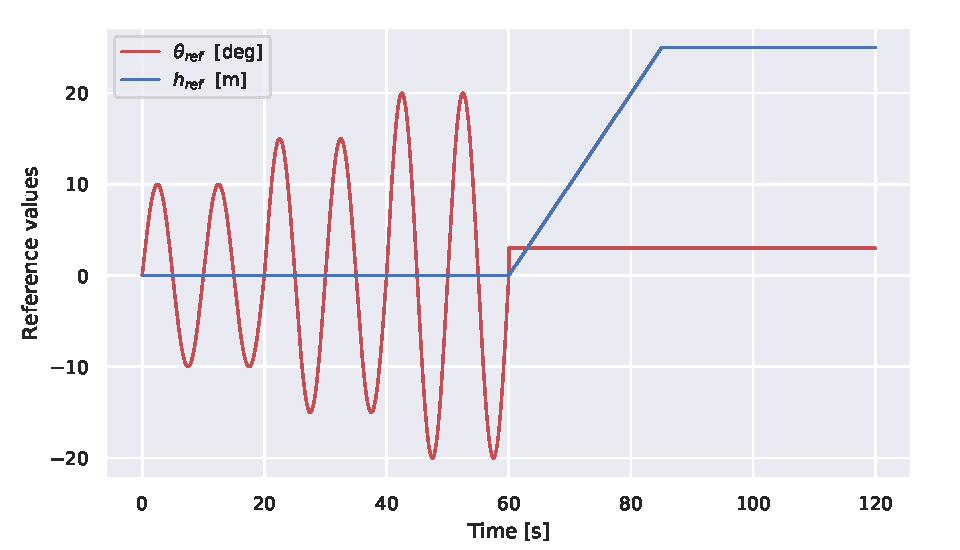
\includegraphics[width=0.9\textwidth]{fig/4/reference_training.pdf}
    \caption[]{Reference pitch angle and altitude during the training scenario}
    \label{fig:reference_training}
\end{figure}

It can be seen that the pitch angle reference signal amplitude $A_{ref}$ increases in steps over the first minute of training time, starting at $10\si{\degree}$, increasing to $15\si{\degree}$ after 20 seconds, and $20\si{\degree}$ after 40 seconds. This approach was found to lower the chance of the agent overshooting the reference significantly when provided with a very large tracking error early in training.
After 60 seconds, the learning rate of the cyclic agent is reduced by 90\%, the collective PID controller is switched off, and the collective RL agent starts training. The learning task of the collective agent is a steady climb with a climb rate of 2$\si[per-mode=symbol]{\meter \per \second}$ for 30 seconds, followed by an altitude hold for 30 seconds. Meanwhile, the cyclic is asked for a constant pitch angle $\theta_{ref} = 2.5\si{\degree}$ to steadily reduce forward airspeed. At the end of the training run, the helicopter should be at steady altitude and approximately zero airspeed. 

To help with the incremental model identification, an exponentially decaying sinusoidal excitation is applied to both inputs in the first eight seconds. A sine signal was preferred over other common excitation patterns such as 3211 or doublet because it exposes the model to different action increments as well as different state increments each timestep, allowing for more rapid convergence. 

The optimal hyperparameters for training were found by means of a grid search. Each combination of parameters was tested for 100 trials, and the success rate and final performance of each experiment was measured. The final performance is measured in the root-mean-squared error (RMSE) of the final 10 seconds of the experiment. Those hyperparameters with the best combination of success rate and final performance were used to train one agent whose weights were then saved and used as a starting point for the maneuvers in the test phase.

\subsection{Test phase} \label{ssec:testphase}

The test phase consisted of two maneuvers aimed at pushing different parts of the longitudinal envelope. Both maneuvers are initialized from a pre-trained agent, but with 90\% reduced learning rates with respect to the training scenario. 

The first manoeuvre was a modified ADS-33 \cite{ADS33} acceleration-deceleration. Its objective is to check the heave and pitch axis for aggressive maneuvering near the rotorcraft limits of performance, undesirable longitudinal-lateral coupling, and harmony between the pitch and heave controls. The desired performance characteristics are as follows. From hover, the aircraft accelerates to $25\si[per-mode=symbol]{\meter \per \second}$ using maximum power while maintaining altitude and lateral track deviations below 15 and 3 meters, respectively. After attaining the target speed, an immediate deceleration takes place, achieving at least $30\si{\degree}$ pitch-up attitude and less than 5\% engine power. 

The second manoeuvre was a one-engine inoperative landing based on \cite{Gille2006}. This manoeuvre checked the controller for the ability to quickly adapt to a new trim point, perform steady flight for a while, followed by an immediate aggressive manoeuvre under reduced engine power. A single engine failure occurred at low altitude, after which the helicopter no longer had enough power to perform a balked landing. Therefore a continuous landing with flare manoeuvre was performed. The safe limits of forward and downward velocity during touchdown, $u_{max}$ and $w_{max}$, were assumed to be 4.5$\si[per-mode=symbol]{\meter \per \second}$ and 1.5$\si[per-mode=symbol]{\meter \per \second}$, respectively \cite{OEILandings}.